\chapter{Introdução}
\label{chap:intro}
\begin{flushright}
	"Faça ou não faça, tentativa não há." \\
	\ \\
	(Mestre Yoda)
\end{flushright}

Quando se ouve falar em robôs, logo associa-se a algo de extrema complexidade. Isso ocorre, sumariamente, devido à falta de informações simplificadas sobre o tema, ou devido a dificuldade de acesso a tais conteúdos. A palavra robótica é derivada da palavra robô, que, segundo \cite{goncalves2007}, é um dispositivo eletromecânico capaz de realizar tarefas de maneira autônoma ou pré-programada, e faz menção a ciência que estuda, cria e aplica robôs. 
No meio educacional, a palavra didática está presente de forma quase que impreterível, afinal, materiais didáticos, livros, projetos e a própria didática como um instrumento qualificador do professor, são componentes fundamentais do cotidiano educacional. Porém é notório que barreiras na educação da atualidade estão sendo quebradas, onde o estudante deixa de frequentar as salas de aula, tornando assim o professor apenas um facilitador do aprendizado do aluno, um tutor. A tutoria é um método muito utilizado para efetivar uma interação pedagógica. Segundo \cite{sa1998}, na educação à distância, o tutor recebe o significado de "orientador de aprendizagem do aluno solitário e isolado".
O sistema de tutoria torna mais fácil o acesso do aluno ao conhecimento, pois o professor passa a ser apenas um orientador, desta maneira aluno torna-se independente na busca das informações, assim, simplificando o aprendizado do aluno. Percebendo essa nova dinâmica da educação, e a falta de informações simplificadas sobre robótica, notou-se a possibilidade de criar um kit didático, para incentivar as pessoas através de desafios e simplificar as informações em torno da robótica.

%-------New Section-----------

\section{Objetivos}
\subsection{Objetivo Geral}
Projetar um kit didático de aprendizagem de conceitos básicos em robótica aplicada, utilizando o framework ROS e aplicando conceitos básicos de cinemática e visão computacional.

\subsection{Objetivos Específicos}
\begin{itemize}
	\item Projetar e fabricar componentes de hardware e peças para aplicação prática do kit;
	\item Desenvolver guias e tutoriais sobre robótica e sobre a utilização do kit;
	\item Construir programas modelos para fácil assimilação e tutoriais de alteração dos programas.
	
\end{itemize}

%-----------New Section----------------------
\section{Justificativa}
Ultimamente, segundo o resumo executivo World Robotics 2018 Robôs Industriais da International Federation of Robotics\cite{ifr2018}, houve uma crescente utilização de sistemas robóticos e autônomos na nossa sociedade. A demanda global de robôs tem crescido severamente, com estimativa de acréscimo de 14\% ao ano até 2021, como visto na figura~\ref{fig:just_1}.

\begin{figure}[h!]										\caption{Estimativa anual de produção global de robôs até o ano de 2021} \label{fig:just_1}		
	\centering										
	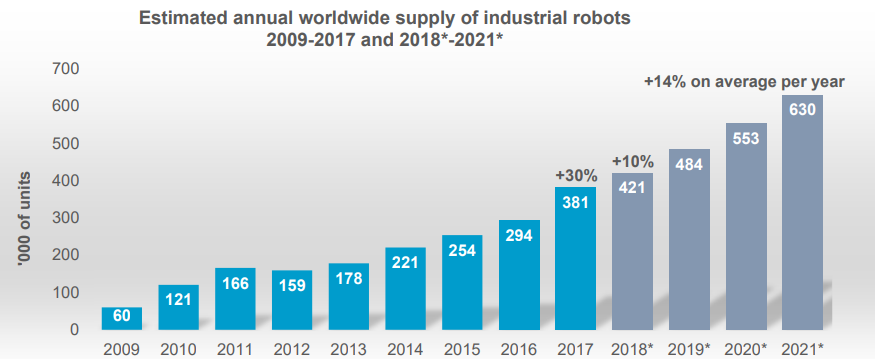
\includegraphics[width=0.5\textwidth]{just_1.PNG}
	\source{\cite{ifr2018}}		
\end{figure}

\begin{figure}[h!]										\caption{Demanda global de robôs em cada setor da indústria no período 2015-2017} \label{fig:just_2}		
	\centering										
	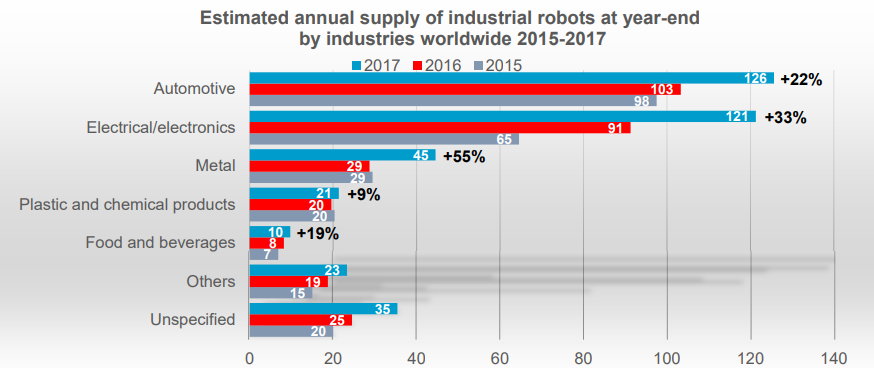
\includegraphics[width=0.5\textwidth]{just_2.PNG}
	\source{\cite{ifr2018}}		
\end{figure}

Esse aumento na demanda está presente em todas as áreas da indústria, como mostrado na figura ~\ref{fig:just_2}, com maior relevâncias nos setores eletroeletrônico e automotivo, de onde vêm as maiores expectativas de inovação por parte da população. Um exemplo de tecnologia que está sendo desenvolvida nessa área, e que é uma das mais esperadas pelo público, são os carros autônomos, que prometem, além da condução independente, maior segurança para os passageiros e tomadas de decisões importantes como a escolha de rotas e ações para evitar acidentes.
Aliado a isso, existe um aumento na demanda por profissionais qualificados cada vez maior nesse setor. Em adição, há ainda uma notória dificuldade em capacitar trabalhadores para lidar com tecnologias as quais eles não tiveram contato durante o ensino médio e fundamental. Alguns conceitos, que não são novos, como sistemas autônomos, machine learning, big data, tem despertado a curiosidade e estimulando a imaginação da sociedade. Porém, isso vem trazendo alguns equívocos.
Um dos problemas encontrados na formação de profissionais para atuar na área, é que, diante destes “novos” conceitos as pessoas tendem a se retrair e ter uma noção equivocada, pensando que estes conceitos, que são primordiais para robótica, são extremamente difíceis e complexos, quando na verdade a abordagem de ensino não se preocupa com a desmistificação destes conceitos.
É comum ouvir que a automação irá estabelecer novas relações trabalhistas, irá extinguir alguns empregos e irá criar outros, porém, será que a nossa sociedade está preparada para estes novos empregos? 
Analisando a conjuntura atual, uma nova abordagem ao ensino de conceitos básicos de robótica foi idealizada, sendo apresentada como um kit didático de robótica básica aplicada. Este kit terá como principal objetivo o ensino teórico e prático, de conceitos e ferramentas básicas utilizadas no mundo da robótica, em aplicações nos mais diversos setores da sociedade. 


%--------- NEW SECTION ----------------------
\section{Organização do \thetypework}
\label{section:organizacao}
O documento está organizado em cinco capítulos, seguindo a seguinte estrutura:

\textbf{Capitulo 1 - Introdução}: Faz a contextualização do âmbito no qual a pesquisa proposta
está inserida. Apresenta, portanto, a problemática, objetivos e como este projeto Theoprax de conclusão de curso está estruturado


\textbf{Capítulo 2 - Referencial Teórico}: Apresenta a base teórica necessária para o desenvolvimento do projeto.

\textbf{Capítulo 3 - Metodologia}: Define o método adotado para o desenvolvimento do projeto, explicitando seu fluxo de atividades e premissas necessárias para aplicar a metodologia.

\textbf{Capítulo 4 - Desenvolvimento}: Exibe os procedimentos realizados e resultados obtidos através de testes, unitários e integrados, durante o desenvolvimento do projeto.

\textbf{Capítulo 5 - Conclusão}: Apresenta as conclusões, contribuições e algumas sugestões de atividades de pesquisa a serem desenvolvidas futuramente.
